% Template for Cogsci submission with R Markdown

% Stuff changed from original Markdown PLOS Template
\documentclass[10pt, letterpaper]{article}

\usepackage{cogsci}
\usepackage{pslatex}
\usepackage{float}
\usepackage{caption}

% amsmath package, useful for mathematical formulas
\usepackage{amsmath}

% amssymb package, useful for mathematical symbols
\usepackage{amssymb}

% hyperref package, useful for hyperlinks
\usepackage{hyperref}

% graphicx package, useful for including eps and pdf graphics
% include graphics with the command \includegraphics
\usepackage{graphicx}

% Sweave(-like)
\usepackage{fancyvrb}
\DefineVerbatimEnvironment{Sinput}{Verbatim}{fontshape=sl}
\DefineVerbatimEnvironment{Soutput}{Verbatim}{}
\DefineVerbatimEnvironment{Scode}{Verbatim}{fontshape=sl}
\newenvironment{Schunk}{}{}
\DefineVerbatimEnvironment{Code}{Verbatim}{}
\DefineVerbatimEnvironment{CodeInput}{Verbatim}{fontshape=sl}
\DefineVerbatimEnvironment{CodeOutput}{Verbatim}{}
\newenvironment{CodeChunk}{}{}

% cite package, to clean up citations in the main text. Do not remove.
\usepackage{apacite}

% KM added 1/4/18 to allow control of blind submission


\usepackage{color}

% Use doublespacing - comment out for single spacing
%\usepackage{setspace}
%\doublespacing


% % Text layout
% \topmargin 0.0cm
% \oddsidemargin 0.5cm
% \evensidemargin 0.5cm
% \textwidth 16cm
% \textheight 21cm

\title{Quantifying social information in natural infant visual experience}


\author{{\large \bf Bria Long (bria@stanford.edu)}  \AND {\large \bf George Kachergis (kachergis@stanford.edu)}  \AND {\large \bf Ketan Jay Agarwal (agrawalk@stanford.edu)}  \AND {\large \bf Michael C. Frank (mcfrank@stanford.edu)} \\ Department of Psychology, Street Address \\ Stanford, CA 91305 USA}

\begin{document}

\maketitle

\begin{abstract}
Faces are a critical part of infants' visual experience, as they convey
social and linguistic information.

\textbf{Keywords:}
Add your choice of indexing terms or keywords; kindly use a semi-colon;
between each term.
\end{abstract}

\hypertarget{introduction}{%
\section{Introduction}\label{introduction}}

Previous work has suggested: - Relative changes in prevalence of faces
vs.~hands (Fausey 2016), though perhaps this is driven by infants
younger than 4 months of age (e.g., Jayaraman, Fausey, \& Smith, 2015;
Sugden, Mohamed-Ali, \& Moulson, 2014) who see both more frequent and
more persistent faces (Jayaraman \& Smith, 2018)

\begin{itemize}
\item
  Surprising attention to hand movements and their interactions with
  objects (Yu \& Smith, 2013), particularly in older infants
\item
  Differences in the availability of social information depending on
  motor abilities (Sanchez, Long et al., 2018 CogSci; Franchack papers)
\end{itemize}

One limitation of past work is that it has relied on cross-sectional
data, and thus cannot speak to whether these trajectories are present in
individual children.

Here, we analyze a longitudinal corpus of head-mounted camera data,
leveraging over XX hours of videos from XX children, totaling more than
XX frames. \{briefly describe dataset; sampling strategy: location of
two households, number of hours of video, variability in location, etc;
reference published paper on what this dataset is, large field of view
(fisheye lens))

To do so, we first test and validate novel computer vision methods for
extracting social information from these egocentric viewpoints on a
small subset of randomly selected frames from the dataset. We then apply
these methods at scale to the larger dataset, allowing us to extract key
descriptive variables hypothesized to vary across development.

Part 1: How well can we capture social information using computer
vision? - Description of OpenPose (Figure 1) - Description of annotation
strategy (24K by Ketan, \textasciitilde{}4K on turk, reliability) -
Describe main P/R/F statistics for 24K for faces and hands; interpret.
Relatively higher precision vs.~recall. - P/R/F variation across
child/age for faces - Describe possible sources of variation that
decrease scores for: - Faces: weird viewpoints, occluded/side viewpoint,
faces in books - Hands: children's own hands, hands in books, side
viewpoints - Describe additional child vs.~hand annotation; P/R/F
variation across child vs.~adult hands (better for adult hands, still OK
for child hands)

Part 2: Access to social information across age Prevalence of hands vs
faces across age (in goldset, full dataset) (Figure 2) Why so many
hands? More child hands as in gold set Cropped analysis

Variation across location contexts (goldset, full dataset)

\hypertarget{method}{%
\section{Method}\label{method}}

If the authors' names are included in the sentence, place only the year
in parentheses, as in (2011), but otherwise place the entire reference
in parentheses with the authors and year separated by a comma (Fausey,
Jayaraman, \& Smith, 2016). List multiple references alphabetically and
separate them by semicolons (Frank, 2012; Smith, Yu, \& Pereira, 2011).
Use the et. al.~construction only after listing all the authors to a
publication in an earlier reference and for citations with four or more
authors.

You might want to display a wide figure across both columns. To do this,
you change the \texttt{fig.env} chunk option to \texttt{figure*}. To
align the image in the center of the page, set \texttt{fig.align} option
to \texttt{center}. To format the width of your caption text, you set
the \texttt{num.cols.cap} option to \texttt{2}.

\hypertarget{one-column-images}{%
\subsection{One-column images}\label{one-column-images}}

Single column is the default option, but if you want set it explicitly,
set \texttt{fig.env} to \texttt{figure}. Notice that the
\texttt{num.cols} option for the caption width is set to \texttt{1}.

\begin{CodeChunk}
\begin{figure}[H]

{\centering 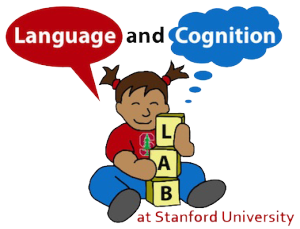
\includegraphics{figs/image-1} 

}

\caption[One column image]{One column image.}\label{fig:image}
\end{figure}
\end{CodeChunk}

\hypertarget{r-plots}{%
\subsection{R Plots}\label{r-plots}}

You can use R chunks directly to plot graphs. And you can use latex
floats in the fig.pos chunk option to have more control over the
location of your plot on the page. For more information on latex
placement specifiers see
\textbf{\href{https://en.wikibooks.org/wiki/LaTeX/Floats,_Figures_and_Captions}{here}}

\begin{CodeChunk}
\begin{figure}[H]

{\centering 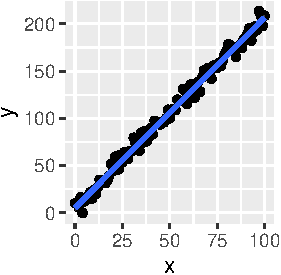
\includegraphics{figs/plot-1} 

}

\caption[R plot]{R plot}\label{fig:plot}
\end{figure}
\end{CodeChunk}

\hypertarget{tables}{%
\subsection{Tables}\label{tables}}

You can use the xtable function in the xtable package.

\begin{table}[H]
\centering
\begin{tabular}{rrrrr}
  \hline
 & Estimate & Std. Error & t value & Pr($>$$|$t$|$) \\ 
  \hline
(Intercept) & 0.00 & 0.10 & 0.0 & 0.98 \\ 
  x & 1.90 & 0.09 & 20.1 & 0.00 \\ 
   \hline
\end{tabular}
\caption{This table prints across one column.} 
\end{table}

\hypertarget{discussion}{%
\section{Discussion}\label{discussion}}

Fausey 2016: 103,383 images; Here: 30,000,000 frames; 300 fold increase
in data

\hypertarget{acknowledgements}{%
\section{Acknowledgements}\label{acknowledgements}}

We would like to thank X and Y for helpful comments, and\ldots{}

\hypertarget{references}{%
\section{References}\label{references}}

\setlength{\parindent}{-0.1in} 
\setlength{\leftskip}{0.125in}

\noindent

\hypertarget{refs}{}
\leavevmode\hypertarget{ref-Fausey2016}{}%
Fausey, C. M., Jayaraman, S., \& Smith, L. B. (2016). From faces to
hands: Changing visual input in the first two years. \emph{Cognition},
\emph{152}, 101--107.

\leavevmode\hypertarget{ref-Franchak2011}{}%
Franchak, J. M., Kretch, K. S., Soska, K. C., \& Adolph, K. E. (2011).
Head-mounted eye- tracking: A new method to describe infant looking.
\emph{Child Development}, \emph{82}(6), 1738--1750.

\leavevmode\hypertarget{ref-Frank2012}{}%
Frank, M. C. (2012). Measuring children's visual access to social
information using face detection. In \emph{Proceedings of the nth annual
conference of the cognitive science society} (pp. XXX--XXX). Hillsdale,
NJ: Cognitive Science Society.

\leavevmode\hypertarget{ref-Smith2011}{}%
Smith, L. B., Yu, C., \& Pereira, A. (2011). Not your mother's view: The
dynamics of toddler visual experience. \emph{Developmental Science},
\emph{14}(1), 9--17.

\bibliographystyle{apacite}


\end{document}
